\documentclass{article}

%% doc settings
\hyphenchar\font=-1 % suppress hyphenation
\setlength\parindent{0pt} % suppress indentation
\usepackage[margin=1.25truein]{geometry} % set page margins

%% libraries 
\usepackage{listings}
\usepackage{fancyhdr}
\usepackage{lastpage}
\usepackage{url}
\usepackage{xcolor}
\usepackage{hyperref}
\usepackage{amssymb}
\usepackage{amsthm}
\usepackage{amsmath}
\usepackage{algorithm}
\usepackage{algcompatible}
\usepackage{natbib}
\usepackage{tikz}
\usepackage{pgfplots}
\usepackage{textcomp}
\usepackage{subcaption}
\usetikzlibrary{shapes, arrows}

%% link viz
\hypersetup{
    colorlinks = true,
    linkcolor = red,
    urlcolor = red,
    citecolor = black
}

%% code colors 
\definecolor{codegreen}{rgb}{0,0.6,0}
\definecolor{codegray}{rgb}{0.5,0.5,0.5}
\definecolor{codepurple}{rgb}{0.58,0,0.82}
\definecolor{backcolour}{rgb}{0.95,0.95,0.92}

\lstdefinestyle{mystyle}{
    backgroundcolor=\color{backcolour},   
    commentstyle=\color{codegreen},
    keywordstyle=\color{magenta},
    numberstyle=\tiny\color{codegray},
    stringstyle=\color{codepurple},
    basicstyle=\ttfamily\footnotesize,
    breakatwhitespace=false,         
    breaklines=true,                 
    captionpos=b,                    
    keepspaces=true,                 
    numbers=left,                    
    numbersep=5pt,                  
    showspaces=false,                
    showstringspaces=false,
    showtabs=false,                  
    tabsize=2
}

\lstset{style=mystyle}

%% math ops
\DeclareMathOperator*{\argmax}{argmax} % thin space, limits underneath in displays

%% page nums
\pagestyle{fancy}
\fancyhf{}
\fancyfoot[C]{Pg. \thepage \space of \pageref*{LastPage}}
\renewcommand{\headrulewidth}{0pt}

%% begin doc
\begin{document}
\title{SYSEN 6000: Foundations of Complex Systems\\~\\
    \Large Machine Learning
}
\author{
    Nick Kunz [NetID: \url{nhk37}] \hyperlink{nhk37@cornell.edu}{nhk37@cornell.edu}}
\date{November 18, 2022}
\maketitle
\thispagestyle{fancy}

%% body doc
\section*{Data Set}
Given a data set $D_{n \times m}$, where $n$ is the number of observations and $m$ is the number of feature vectors $X_1, X_2, X_3, \ldots, X_m$, with target label $Y$, where all $X_i, Y \in D_{n \times m}$, and $D_{test}$ is the test sample $D_{1 \times m}$, where $Y \notin D_{test}$, the following is:

\begin{center}
    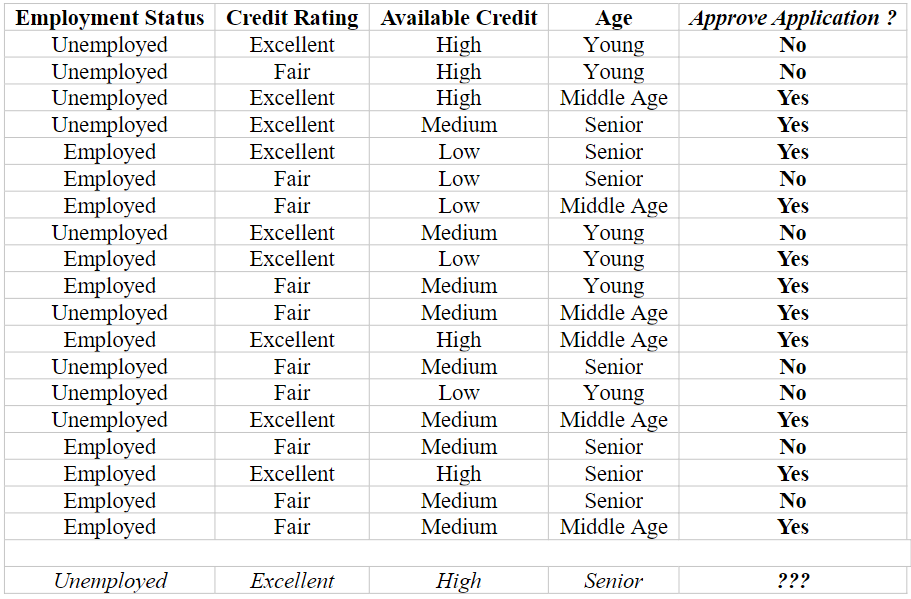
\includegraphics[width=0.90\textwidth]{data.png}
\end{center}

where $n = 19$, $m = 4$ and:
\begin{equation}
\begin{split}
    X_1 & = $Employment Status$\\
    X_2 & = $Credit Rating$\\
    X_3 & = $Available Credit$\\
    X_4 & = $Age$\\
    Y & = $Approve Application?$
\end{split}
\end{equation}

\break
\item \textbf{Implementation}\\
The script for the give data set $D_{n \times m}$ and test sample $D_{test}$ is as follows:

\begin{lstlisting}[language=Python, title=Python 3: Data Set \& Test Sample]
## features
var = [
    'Employment Status',
    'Credit Rating',
    'Available Credit',
    'Age',
    'Approve Application'
]

## observations
obs = [
    ['Unemployed', 'Excellent', 'High', 'Young', 'No'],
    ['Unemployed', 'Fair', 'High', 'Young', 'No'],
    ['Unemployed', 'Excellent', 'High', 'Middle Age', 'Yes'],
    ['Unemployed', 'Excellent', 'Medium', 'Senior', 'Yes'],
    ['Employed', 'Excellent', 'Low', 'Senior', 'Yes'],
    ['Employed', 'Fair', 'Low', 'Senior', 'No'],
    ['Employed', 'Fair', 'Low', 'Middle Age', 'Yes'],
    ['Unemployed', 'Excellent', 'Medium', 'Young', 'No'],
    ['Employed', 'Excellent', 'Low', 'Young', 'Yes'],
    ['Employed', 'Fair', 'Medium', 'Young', 'Yes'],
    ['Unemployed', 'Fair', 'Medium', 'Middle Age', 'Yes'],
    ['Employed', 'Excellent', 'High', 'Middle Age', 'Yes'],
    ['Unemployed', 'Fair', 'Medium', 'Senior', 'No'],
    ['Unemployed', 'Fair', 'Low', 'Young', 'No'],
    ['Unemployed', 'Excellent', 'Medium', 'Middle Age', 'Yes'],
    ['Employed', 'Fair', 'Medium', 'Senior', 'No'],
    ['Employed', 'Excellent', 'High', 'Senior', 'Yes'],
    ['Employed', 'Fair', 'Medium', 'Senior', 'No'],
    ['Employed', 'Fair', 'Medium', 'Middle Age', 'Yes']
]

## predictions
test = ['Unemployed', 'Excellent', 'High', 'Senior']\end{lstlisting}\\

\section*{Decision Tree Classifier}
The following is an exhibit of a Decision Tree classifier utilizing Entropy and Information Gain for the given data set $D_{n \times m}$ and $D_{test}$, where Entropy is computed as:
\begin{equation}
    H(X) = - \sum_{j=1}^{c}p_j \log_2 (p_j)
\end{equation}\\
and $p_j$ is the probability of observing class $C$, which can also be expressed as:
\begin{equation}
    H(X) = \sum_{j=1}^{c} \log_2 \left( \frac{1}{p_j} \right) p_j
\end{equation}


Information Gain is computed as:
\begin{equation}
    IG (Y, X) = H(Y) - H(Y|X)
\end{equation}\\

\break
Building the Decision Tree classifier utilizing Information Gain occurs in these steps.

\begin{algorithm}
\caption{Decision Tree Classifier}
\textbf{Input: $D_{n \times m}$, $D_{test}$}\\
\textbf{Output:} class $C$ of $D_{test}$
\begin{algorithmic}[1]
    \FOR{each $i$}
        \STATE compute $IG(Y, X_i)$
    \item \textbf{end for}
    \item create node $N_i$ with highest $IG$
    \item \textbf{if} all $Y_j \in N_i$ are the same class $C$, \textbf{then}
        \STATE \textbf{return} leaf node labeled class $C$ to tree
    \item \textbf{else} step 1
    \item \textbf{end if}
    \item \textbf{if} tree is \textbf{done}, \textbf{then}
        \STATE traverse $N_i$ in tree with $X_{j \times m} \in D_{test}$ until $C$
        \STATE \textbf{return} leaf node as class $C$
    \item \textbf{end if}
    
\end{algorithmic}
\end{algorithm}

\item \textbf{Implementation}\\
The scripts for the Decision Tree classifier are as follows:
\begin{lstlisting}[language=Python, title=Python 3: Decision Tree Classifier]
## libraries
import math
import pprint

## feat vect of data
def feat_vect(x_y, y_i):
    
    n = len(x_y)

    return [x_y[i][y_i] for i in range(0, n)]


## feat subset of data
def feat_subs(x_y, y_i):

    n = len(x_y)

    return [x_y[i][0:y_i] for i in range(0, n)]


## count unique vals of feat
def counter(y_j):

    ## find unique vals
    uni_val = list(
        set([j for j in y_j])
    )

    ## count unique vals
    uni_val_cts = dict.fromkeys(
        uni_val, 0
    )

    n = len(y_j)
    i_j = [None] * n

    for j in range(0, n):
        i_j[j] = y_j[j]

    for i in i_j:
        uni_val_cts[i] += 1

    return uni_val_cts


## entropy of feat
def entropy(y_j):

    ## count unique vals
    cts = counter(
        y_j = y_j
    )

    ## compute probs
    n = len(y_j)

    prob = [(j / n) for j in cts.values()]

    ## compute entropy
    return sum(
        [-p * math.log(p, 2) for p in prob]
    )


## info gain of data
def info_gain(x_y, x_i, y_i):

    ## trgt feat
    y_j = feat_vect(
        x_y = x_y, 
        y_i = y_i
    )

    ## attr feat
    x_a = feat_vect(
        x_y = x_y, 
        y_i = x_i
    )

    ## count unique vals
    cts = counter(
        y_j = x_a
    )

    ## comp entropy
    entp = entropy(
        y_j = y_j
    )

    ## cond entropy of feat
    entp_cond = 0

    for i, uni in enumerate(cts):

        ## subset data by unique vals in trgt feat
        x_y_uni = [j for j in x_y if j[x_i] == uni]

        ## attr feat of subset
        y_v = feat_vect(
            x_y = x_y_uni, 
            y_i = y_i
        )

        ## cond entropy of attr feat
        entp_cond += (cts[uni] / len(x_a)) * entropy(
            y_j = y_v
        )

    ## info gain
    return entp - entp_cond


## decision tree on data
def grow_tree(x_y, y_i, tree = None):

    ## feat info gain
    m = len(x_y[0]) - 1
    info = [None] * m

    for i in range(0, m):
        info[i] = info_gain(
            x_y = x_y, 
            x_i = i,
            y_i = y_i
        )

    ## best feat split
    x_i_star = info.index(max(info))

    x_i_feat = feat_vect(
        x_y = x_y, 
        y_i = x_i_star
    )

    x_i_splt = counter(
        y_j = x_i_feat
    )

    if tree is None:
        tree = dict()
        tree[x_i_star] = dict()
    
    else:
        pass

    ## cont feat split
    n = len(x_y)

    for i in x_i_splt:
        x_y_splt = list()
        
        for j in range(0, n):
            if x_y[j][x_i_star] == i:
                x_y_splt.append(x_y[j])

        y_j = [x_y_splt[k][y_i] for k in range(0, len(x_y_splt))]
        y_j_freq = counter(
            y_j = y_j
        )
            
        ## leaf node
        if len(y_j_freq) == 1:
            tree[x_i_star][i] = y_j_freq

        ## recursion
        else:
            tree[x_i_star][i] = grow_tree(
                x_y = x_y_splt, 
                y_i = y_i
            )

    return tree


## predict on decision tree dict
def pred_tree(tree, test, verb = False):

    k = list(tree.keys())[0]
    v = list(tree.values())[0]

    if isinstance(v, dict) == True:
        if verb == True:
            print(test[k])

        return pred_tree(
            tree = v[test[k]],
            test = test,
            verb = verb
        )
    else:
        return k

## decision tree
tree = grow_tree(
    x_y = obs,
    y_i = 4
)

## prediction
pred_tree(
    tree = tree,
    test = test
)\end{lstlisting}
\verb|"Yes"|\\


\begin{lstlisting}[language=Python, title=Python 3: Decision Tree]
## view tree
pprint.pprint(tree)\end{lstlisting}
\verb|{3: {'Middle Age': {'Yes': 6}, |\\
\verb|     'Senior': {1: {'Excellent': {'Yes': 3}, 'Fair': {'No': 4}}}, |\\
\verb|     'Young': {0: {'Employed': {'Yes': 2}, 'Unemployed': {'No': 4}}}}} |\\

\break

\section*{Naive Bayes Classifier}
The following is an exhibit of a Naive Bayes classifier assuming independence for the given data set $D_{n \times m}$ and $D_{test}$, where Bayes theorem is computed as:\\
 
\begin{equation}
    P(X|Y) = \frac{P(Y|X) P(X)}{P(Y)}
\end{equation}

which assumes independence, such that:
\begin{equation}
    P(X_1, X_2, X_3, \ldots, X_m|Y) = \prod_{i = 1}^{m} P(X_i|Y)
\end{equation}\\

where $X_i$ and $X_j$ are conditionally independent on $Y$, such that:

\begin{equation}
    \forall \, i \neq j
\end{equation}\\
which implies that a classifier can be expressed as:
\begin{equation}
    P(C_k | X) = \frac{P(C_k)P(X|C_k)}{P(X)} = \frac{P(C_k) \prod_{i = 1}^{m} P(X_i|C_k)}{P(X)}
\end{equation}\\

where $k$ is a class $C$, and $C$ can be estimated by:\\
\begin{equation}
    \hat{C} = \argmax_{k \in K} P(C_k) \prod_{i = 1}^{m} P(X_i|Y)
\end{equation}\\

Building the Naive Bayes classifier assuming independence occurs in these steps.
\begin{algorithm}
\caption{Naive Bayes Classifier}
\textbf{Input: $D_{n \times m}$, $D_{test}$}\\
\textbf{Output:} class $C$ of $D_{test}$
\begin{algorithmic}[1]
    \FOR{each $k$}
        \STATE compute $P(C_k)$
        \FOR{each $i$}
            \STATE compute $P(X_i|C_k)$
        \ENDFOR
    \item \textbf{end for}
    \item \textbf{return} $\argmax_{k\in K}P(C_k)\prod_{i=1}^{m}P(X_i|C_k)$
\end{algorithmic}
\end{algorithm}

\item \textbf{Implementation}\\
The scripts for the Naive Bayes classifier are as follows:
\begin{lstlisting}[language=Python, title=Python 3: Naive Bayes Classifier]
## class prob
def class_prob(y_j):

    ## count unique vals
    y_j_cts = counter(
        y_j = y_j
    )

    y_i_prob = y_j_cts.copy()

    n = len(y_j)

    for i in y_j_cts.keys():
        y_i_prob[i] = round(
            number = (y_j_cts[i] / n),
            ndigits = 3
        )

    return y_i_prob


## conditional prob
def cond_prob(x_y, y_i):

    ## trgt feat
    y_j = feat_vect(
        x_y = x_y, 
        y_i = y_i
    )

    ## count unique vals
    cts = counter(
        y_j = y_j
    )

    ## cond prob
    n = len(x_y)
    m = len(x_y[0]) - 1

    y_i_splt = list()
    x_y_cond = cts.copy()

    for i in cts.keys():
        x_y_splt = list()
        x_y_cond[i] = dict()

        for j in range(0, n):
            if x_y[j][y_i] == i:
                x_y_splt.append(x_y[j])

        n_splt = len(x_y_splt)
        
        for j in range(0, m):
            x_splt_subs = feat_vect(
                x_y = x_y_splt,
                y_i = j
            )

            cts_splt_subs = counter(
                y_j = x_splt_subs
            )

            x_splt_prob = {
                k: round(v / n_splt, 3) for k, v in cts_splt_subs.items()
            }
        
            x_y_cond[i].update(x_splt_prob)

    return x_y_cond


## posterior prob
def post_prob(p_clss, p_cond, test):

    post_prob = p_clss.copy()

    for i in p_clss.keys():
        test_prob = 1

        for j in test:
            test_prob = test_prob * p_cond[i][j]

        post_prob[i] = round(
            number = p_clss[i] * test_prob,
            ndigits = 3
        )

    return post_prob


## predict on post prob dict
def pred_post(p_post):

    ## arg max func
    return max(
        p_post,
        key = p_post.get
    )

## class prob
y_j = feat_vect(
    x_y = obs, 
    y_i = 4
)

prob_clss = class_prob(
    y_j = y_j
)

## conditional prob
prob_cond = cond_prob(
    x_y = obs , 
    y_i = 4
)

## posterior prob
prob_post = post_prob(
    p_clss = prob_clss, 
    p_cond = prob_cond, 
    test = test
)

## prediction
pred_post(
    p_post = prob_post
)\end{lstlisting}
\verb|"Yes"|\\

\break
\section*{k-Nearest Neighbors Classifier}
The following is an exhibit of a k-Nearest Neighbors classifier utilizing Jaccard Similarity for the given data set $D_{n \times m}$ and $D_{test}$, where the Jaccard Similarity distance metric is computed as:

\begin{equation}
    J(A | B) = \frac{|A \cap B|}{|A \cup B|}
\end{equation}\\
Building the k-Nearest Neighbors classifier with Jaccard Similarity occurs in these steps.\\
$k$ should be set to an odd number to avoid cases where the number of $C$ in $Y_{j} \in D_{k \times m}$ are equal.
\begin{algorithm}
\caption{k-NN Classifier}
\textbf{Input: $D_{n \times m}$, $D_{test}$}\\
\textbf{Output:} class $C$ of $D_{test}$
\begin{algorithmic}[1]
    \item \textbf{set} $k$ 
    \FOR{each $j$}
        \STATE compute distance $I_j = J(X_{j \times m} | D_{test})$
    \item \textbf{end for}
    \item \textbf{sort} distances $I_j$ in ascending order
    \item \textbf{truncate} $I_j$ by $k$ to $I_k$
    \item \textbf{subset} $D_{n \times m}$ to $D_{k \times m}$ indexed by $I_k$
    \item \textbf{return} majority of $Y_{j} \in D_{k \times m}$ as $C$
\end{algorithmic}
\end{algorithm}

\textbf{Implementation}\\
The scripts for the k-NN classifier are as follows:
\begin{lstlisting}[language=Python, title=Python 3: k-NN Classifier]
## jaccard similiarity
def jaccard(a, b):

    ## intersect
    inter = len(list(set(a).intersection(b)))

    ## union
    n_a, n_b = len(a), len(b)
    union = (n_a + n_b) - inter

    ## proportion
    return round(
        number = inter / union,
        ndigits = 2
    )

## dist matrix on data
def dist_matrix(x_y, y_i, test = False):

    x_i = feat_subs(
        x_y = x_y, 
        y_i = y_i
    )

    n = len(x_i)
    dist_mtrx = [None] * n

    if test is False:
        for i in range(0, n):

            dist = [None] * n

            for j in range(0, n):
                dist[j] = jaccard(
                    a = x_i[i],
                    b = x_i[j]
                )

            dist_mtrx[i] = dist
    
    else:
        for i in range(0, n):
            dist_mtrx[i] = jaccard(
                a = test,
                b = x_i[i]
            )

    return dist_mtrx

## knn on data
def knn(x_y, y_i, k, test = False):
    
    dist_mtrx = dist_matrix(
        x_y = x_y,
        y_i = y_i,
        test = test
    )

    ## find near neigh index
    n = len(dist_mtrx)
    near_negh = dict()

    if test is False:
        for i in range(0, n):

            ## neigh sorted by index
            idx = sorted(
                range(len(dist_mtrx[i])), 
                key = lambda k: dist_mtrx[i][k]
            )

            ## subset near by k
            near_negh[i] = list(
                reversed(idx[-k - 1:][:-1])
            )
    else:
        ## neigh sorted by index
        idx = sorted(
            range(len(dist_mtrx)), 
            key = lambda k: dist_mtrx[k]
        )

        ## subset near by k
        near_negh = list(
            reversed(idx[-k - 1:][:-1])
        )

    return near_negh

## predict on knn test list
def knn_pred(x_y, y_i, k, test):

    idx_knn = knn(
        x_y = x_y,
        y_i = y_i,
        k = k,
        test = test
    )

    n = len(idx_knn)
    x_y_knn = [None] * n

    for i in range(0, n):
        x_y_knn[i] = obs[idx_knn[i]]

    y_j_knn = feat_vect(
        x_y = x_y_knn,
        y_i = y_i
    )

    y_j_hat = counter(
        y_j = y_j_knn
    )

    return max(
        y_j_hat, 
        key = y_j_hat.get
    )\end{lstlisting}

$k = 1$
\begin{lstlisting}[language=Python, title=Python 3: 1-NN Classifier]
## prediction
knn_pred(
    x_y = obs, 
    y_i = 4, 
    k = 1, 
    test = test
)\end{lstlisting}
\verb|"Yes"|\\

$k = 3$
\begin{lstlisting}[language=Python, title=Python 3: 3-NN Classifier]
## prediction
knn_pred(
    x_y = obs, 
    y_i = 4, 
    k = 3, 
    test = test
)\end{lstlisting}
\verb|"No"|\\

$k = 5$
\begin{lstlisting}[language=Python, title=Python 3: 5-NN Classifier]
## prediction
knn_pred(
    x_y = obs, 
    y_i = 4, 
    k = 5, 
    test = test
)\end{lstlisting}
\verb|"Yes"|\\


\break
\section*{Dependency Support Classifiers}
The following verifies the previous details of the given classifiers utilizing common dependencies for machine learning to include: \textit{pandas} and \textit{scikit-learn}. The outputs of the scripts follow the figures.\\

\item \textbf{Data Set}
\begin{lstlisting}[language=Python, title=Python 3: Pandas Dataframe]
## libraries
import pandas as pd
from sklearn.preprocessing import OrdinalEncoder
from sklearn.preprocessing import MinMaxScaler

## data
data = pd.DataFrame(
    data = obs,
    columns = var
)

data_pred = pd.DataFrame(
    data = [test],
    columns = var[0:4]
)

## pre-process
enc = OrdinalEncoder()
mms = MinMaxScaler()

for i in data.columns:
    data[i] = enc.fit_transform(data[[i]])

data = mms.fit_transform(data)
data = pd.DataFrame(
    data = data,
    columns = var
)
data_pred = enc.fit_transform(data_pred)\end{lstlisting}

\item \textbf{Decision Tree Classifier}
\begin{lstlisting}[language=Python, title=Python 3: Scikit-Learn Decision Tree Classifier]
## libraries
from sklearn import tree

## train
clf = tree.DecisionTreeClassifier(
    criterion = 'entropy'
)

clf = clf.fit(
    X = data.drop(['Approve Application'], axis = 1).values,
    y = data['Approve Application']
)

## predict
if int(clf.predict(data_pred)[0]) == 1:
    print('Yes')
else:
    print('No')\end{lstlisting}
\verb|"Yes"|\\


\item \textbf{Naive Bayes Classifier}
\begin{lstlisting}[language=Python, title=Python 3: Scikit-Learn Naive Bayes Classifier]
## libraries
from sklearn.naive_bayes import CategoricalNB

## train
clf = CategoricalNB()

clf = clf.fit(
    X = data.drop(['Approve Application'], axis = 1).values,
    y = data['Approve Application']
)

## predict
if int(clf.predict(data_pred)[0]) == 1:
    print('Yes')
else:
    print('No')\end{lstlisting}
\verb|"Yes"|\\

\item \textbf{k-Nearest Neighbors Classifier}\\

$k = 1$
\begin{lstlisting}[language=Python, title=Python 3: Scikit-Learn 1-NN Classifier]
## libraries
from sklearn.neighbors import KNeighborsClassifier

## train
clf = KNeighborsClassifier(
    n_neighbors = 1,
    metric = 'jaccard'
)

clf = clf.fit(
    X = data.drop(['Approve Application'], axis = 1).values,
    y = data['Approve Application']
)

## predict
if int(clf.predict(data_pred)[0]) == 1:
    print('Yes')
else:
    print('No')\end{lstlisting}
\verb|"Yes"|\\

$k = 3$
\begin{lstlisting}[language=Python, title=Python 3: Scikit-Learn 3-NN Classifier]
## libraries
from sklearn.neighbors import KNeighborsClassifier

## train
clf = KNeighborsClassifier(
    n_neighbors = 3,
    metric = 'jaccard'
)

clf = clf.fit(
    X = data.drop(['Approve Application'], axis = 1).values,
    y = data['Approve Application']
)

## predict
if int(clf.predict(data_pred)[0]) == 1:
    print('Yes')
else:
    print('No')\end{lstlisting}
\verb|"No"|\\

$k = 5$
\begin{lstlisting}[language=Python, title=Python 3: Scikit-Learn 5-NN Classifier]
## libraries
from sklearn.neighbors import KNeighborsClassifier

## train
clf = KNeighborsClassifier(
    n_neighbors = 5,
    metric = 'jaccard'
)

clf = clf.fit(
    X = data.drop(['Approve Application'], axis = 1).values,
    y = data['Approve Application']
)

## predict
if int(clf.predict(data_pred)[0]) == 1:
    print('Yes')
else:
    print('No')\end{lstlisting}
\verb|"Yes"|\\

\textbf{Support Vector Machines Classifier}
\begin{lstlisting}[language=Python, title=Python 3: Scikit-Learn SVM Classifier]
## libraries
from sklearn.svm import SVC

## train
clf = SVC()

clf = clf.fit(
    X = data.drop(['Approve Application'], axis = 1).values,
    y = data['Approve Application']
)

## predict
if int(clf.predict(data_pred)[0]) == 1:
    print('Yes')
else:
    print('No')\end{lstlisting}
\verb|"Yes"|\\


\end{document}